\chapter{Debugging and Testing}

In order to test and debug, ``pytest'' needs to be installed. Once it is installed, it is as simple as calling the pytest with the executable script to run and verify the results. 

\textbf{\textit{Brief description of pytest}}

 It is a test framework written in python to test code written in python.

Very easy to start using the framework and supports to scale complex functional testing.

Community support and documentation is very good.

Supports 150+ plugins.



For our project we used below functionalities which is available in python and part of pytest for tetsing and debugging.

\begin{enumerate}
    \item assertion  [For testing each function, works like "if not" and raises an exception]
    \item fixtures  [For setting up configuration before and then to do clean up after testing is completed] 
    \item pytest.raises [To perform negative testing and to test exceptions] 
    \item conftest [Used to provide the config details and to provide scope of the fixtures]
    \item tox [To create virtual enviranment which provides option to select different verisons of the packages and python versions]
    \item devpi[Repository manager]
\end{enumerate}

The figure \ref{fig:14} displays all the above operation done in python.


\newpage

\begin{figure}[h]
    \centering
    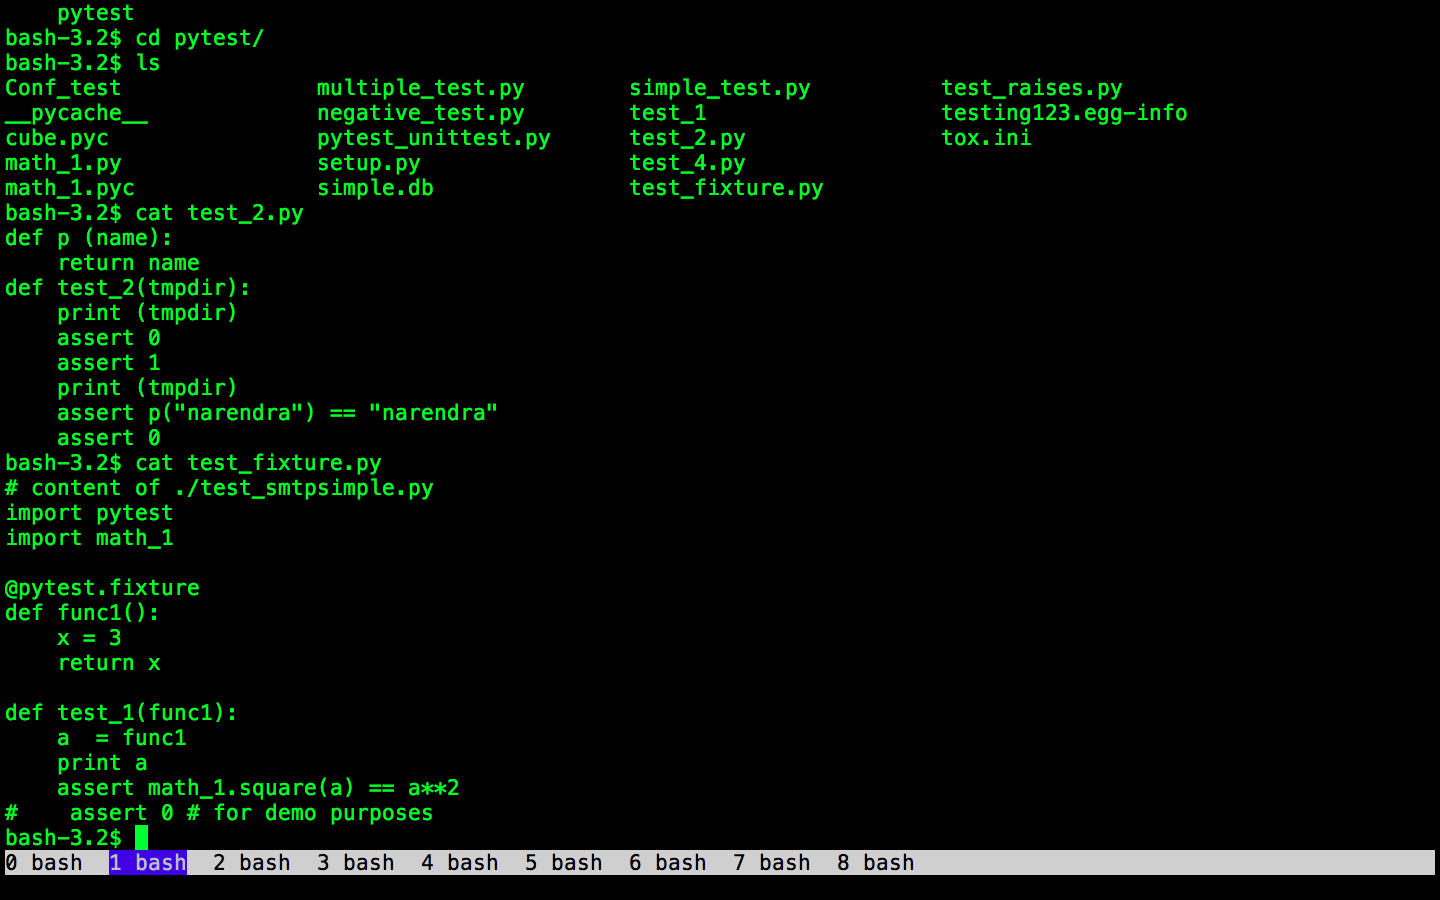
\includegraphics[width=\textwidth]{pytest2}
    \caption{Testing and Debugging in pytest}
    \label{fig:14}
\end{figure}

\newpage